\documentclass[12pt]{article}
\usepackage[table]{xcolor}
\usepackage[shortlabels]{enumitem}
\usepackage{tabularx,xltabular}
\usepackage{graphicx}
\usepackage{hyperref}
\usepackage{verbatim}
\usepackage{geometry}
\usepackage{ulem}
\usepackage[official]{eurosym}
\usepackage{tikz}
\usetikzlibrary{arrows,backgrounds,calc,decorations.markings,patterns,3d}
\usepackage{pgfplots}
\pgfplotsset{compat = newest}
\usetikzlibrary{fit}
\newcommand\addvmargin[1]{
\usetikzlibrary{arrows}
\node[fit=(current bounding box),inner ysep=#1,inner xsep=0]{};}
\usepackage{cancel}
\usepackage{fontspec}
\usepackage{array}  
\geometry{a4paper, top=2cm, left=2cm, right=2cm, bottom=2cm, headsep=1cm}
\usepackage{tabu}
\usepackage{pst-node}
\usepackage{colortbl}
\usepackage{array}
\usepackage{german}
\setlength\parindent{0pt}
\newcolumntype{?}{!{\vrule width 1pt}}
\usepackage{makecell}
\renewcommand{\arraystretch}{2.5}
\usepackage{pbox}
\usepackage{amssymb}
\usepackage{amsmath}
\usepackage{booktabs}
\newcolumntype{L}[1]{>{\raggedright\let\newline\\\arraybackslash\hspace{0pt}}m{#1}}
\newcolumntype{C}[1]{>{\centering\let\newline\\\arraybackslash\hspace{0pt}}m{#1}}
\newcolumntype{R}[1]{>{\raggedleft\let\newline\\\arraybackslash\hspace{0pt}}m{#1}}
\begin{document}
\rightline{Datum: 14.06.2023}
\centerline{{\Large Terme und Gleichungen}} 
\vspace{1cm}
\noindent \\


\begin{xltabular}{\textwidth}{|C{0.75cm}|X|C{0.75cm}|X|}
\arrayrulecolor{black}\hline
a)& $z=3~ \rightarrow ~ 4 \cdot z + z=?$
&
b)& $a=7~ \rightarrow ~ 4 \cdot a - 5=?$
\\\hline
c)& $a=10~ \rightarrow ~ 5 + 3 \cdot a=?$
&
d)& $x=9~ \rightarrow ~ 3 \cdot x - 4=?$
\\\hline
e)&Bestimme ein Term, wenn x=4 und das Ergebnis gleich 0 ist.
&
f)&Bestimme ein Term, wenn x=1 und das Ergebnis gleich -1 ist.
\\\hline
g)&Bestimme ein Term, wenn x=8 und das Ergebnis gleich -64 ist.
&
h)&Bestimme ein Term, wenn x=8 und das Ergebnis gleich 16 ist.
\\\hline
i)&$2 - 4 \cdot y - y + 2 \cdot y$
&
j)&$3 \cdot y + 3 \cdot y + y - 3 \cdot y$
\\\hline
k)&$2 - 2 \cdot y - y$
&
l)&$y + 2 + 2$
\\\hline
m)&$-1\cdot y-18+5+3\cdot y=3$
&
n)&$10\cdot y+5-15-4\cdot y=62$
\\\hline
o)&$-1+1\cdot y-1+1\cdot y=20$
&
p)&$-4+1\cdot y-2+3\cdot y=22$
\\\hline
q)&$-2-1\cdot a+6\cdot a-4=54$
&
r)&$-3\cdot b-7+9\cdot b-13=10$
\\\hline
s)&$-7-6-5\cdot b+11\cdot b=5$
&
t)&$-1+4\cdot x-1+2\cdot x=16$
\\\hline
u)&$8\cdot y+2\cdot y-4-4=82$
&
v)&$5-13-1\cdot y+6\cdot y=17$
\\\hline
w)&$-4\cdot a+14\cdot a+4-23=51$
&
x)&$-5-1\cdot a+4\cdot a-9=-8$
\\\hline
y)&$9\cdot y-12-5-3\cdot y=43$
&
z)&$16\cdot x-14+6-7\cdot x=73$
\\\hline
\end{xltabular}
\vspace{0.5cm}
\newpage
\rightline{Datum: 14.06.2023}
\centerline{{\large Lösungen Terme und Gleichungen}} 
\vspace{0.5cm}

\begin{xltabular}{\textwidth}{|C{0.75cm}|X|C{0.75cm}|X|}
\arrayrulecolor{black}\hline
a)&$\begin{aligned}
\textcolor{red}{z=3} & \rightarrow\\
4 \cdot z + z=&4 \cdot \textcolor{red}{3} + \textcolor{red}{3}=15\\
\end{aligned}$
&
b)&$\begin{aligned}
\textcolor{red}{a=7} & \rightarrow\\
4 \cdot a - 5=&4 \cdot \textcolor{red}{7} - 5=23\\
\end{aligned}$
\\\hline
c)&$\begin{aligned}
\textcolor{red}{a=10} & \rightarrow\\
5 + 3 \cdot a=&5 + 3 \cdot \textcolor{red}{10}=35\\
\end{aligned}$
&
d)&$\begin{aligned}
\textcolor{red}{x=9} & \rightarrow\\
3 \cdot x - 4=&3 \cdot \textcolor{red}{9} - 4=23\\
\end{aligned}$
\\\hline
e)&Ein mögliches Ergebnis:\[ x=4 ~~ \rightarrow x-4=0 \]
&
f)&Ein mögliches Ergebnis:\[ x=1 ~~ \rightarrow -x \cdot 1=-1 \]
\\\hline
g)&Ein mögliches Ergebnis:\[ x=8 ~~ \rightarrow -x \cdot 8=-64 \]
&
h)&Ein mögliches Ergebnis:\[ x=8 ~~ \rightarrow x+8=16 \]
\\\hline
i)&$2 - 4\cdot y - y + 2\cdot y=2 - 3y$
&
j)&$3\cdot y + 3\cdot y + y - 3\cdot y=4y$
\\\hline
k)&$2 - 2\cdot y - y=2 - 3y$
&
l)&$y + 2 + 2=y + 4$
\\\hline
m)&\begingroup\setlength{\jot}{-0.03cm}
\tikzstyle{background grid}=[draw, black!15,step=.5cm]
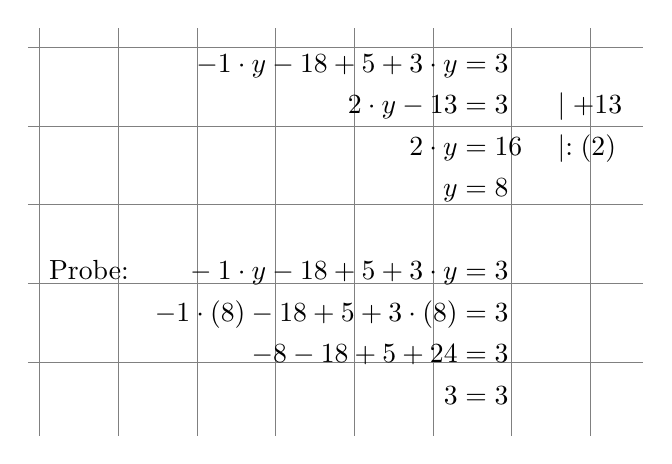
\begin{tikzpicture}[show background grid]
\node[below right] at (0,0.1) {
$\begin{aligned}
-1\cdot y-18+5+3\cdot y &=3& &  \\
2\cdot y - 13 &=3& & \mid + 13\\
2\cdot y &=16& & \mid :\left(2\right)\\
y &=8& & 
\\
\\
\mbox{Probe:}\qquad -1\cdot y-18+5+3\cdot y &=3& &  \\
-1\cdot \left(8\right)-18+5+3\cdot \left(8\right) &=3& &  \\
-8-18+5+24 &=3& &  \\
3 &=3& &  \\
\end{aligned}$};
\end{tikzpicture}
\endgroup
&
n)&\begingroup\setlength{\jot}{-0.03cm}
\tikzstyle{background grid}=[draw, black!15,step=.5cm]
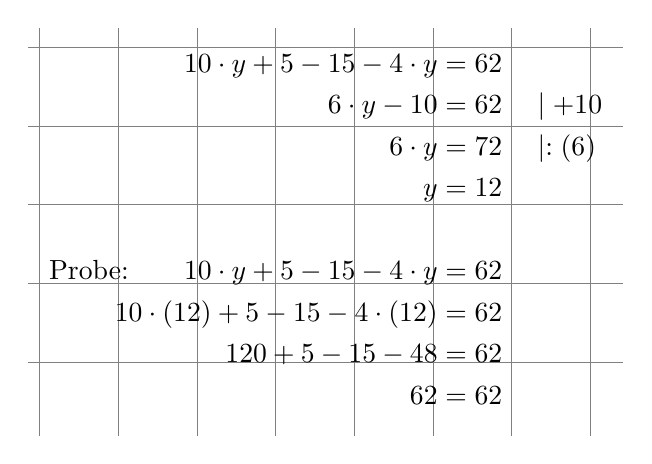
\begin{tikzpicture}[show background grid]
\node[below right] at (0,0.1) {
$\begin{aligned}
10\cdot y+5-15-4\cdot y &=62& &  \\
6\cdot y - 10 &=62& & \mid + 10\\
6\cdot y &=72& & \mid :\left(6\right)\\
y &=12& & 
\\
\\
\mbox{Probe:}\qquad 10\cdot y+5-15-4\cdot y &=62& &  \\
10\cdot \left(12\right)+5-15-4\cdot \left(12\right) &=62& &  \\
120+5-15-48 &=62& &  \\
62 &=62& &  \\
\end{aligned}$};
\end{tikzpicture}
\endgroup
\\\hline
o)&\begingroup\setlength{\jot}{-0.03cm}
\tikzstyle{background grid}=[draw, black!15,step=.5cm]
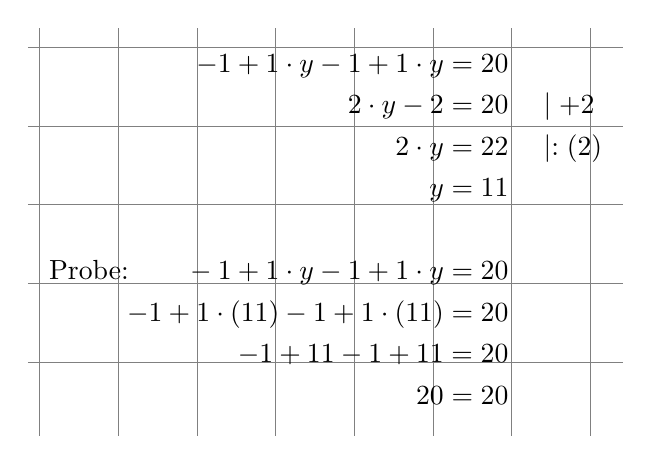
\begin{tikzpicture}[show background grid]
\node[below right] at (0,0.1) {
$\begin{aligned}
-1+1\cdot y-1+1\cdot y &=20& &  \\
2\cdot y - 2 &=20& & \mid + 2\\
2\cdot y &=22& & \mid :\left(2\right)\\
y &=11& & 
\\
\\
\mbox{Probe:}\qquad -1+1\cdot y-1+1\cdot y &=20& &  \\
-1+1\cdot \left(11\right)-1+1\cdot \left(11\right) &=20& &  \\
-1+11-1+11 &=20& &  \\
20 &=20& &  \\
\end{aligned}$};
\end{tikzpicture}
\endgroup
&
p)&\begingroup\setlength{\jot}{-0.03cm}
\tikzstyle{background grid}=[draw, black!15,step=.5cm]
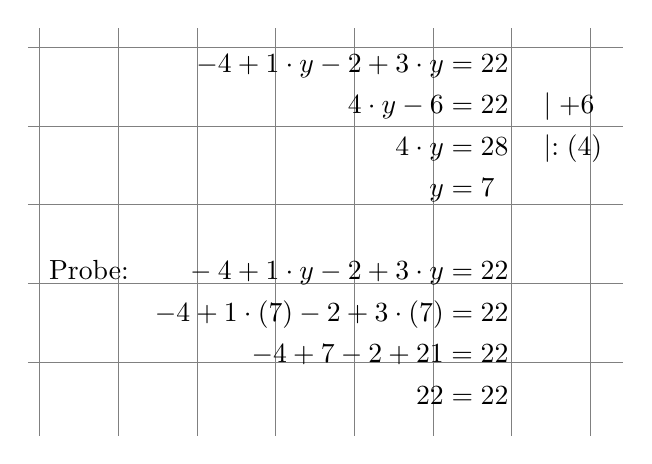
\begin{tikzpicture}[show background grid]
\node[below right] at (0,0.1) {
$\begin{aligned}
-4+1\cdot y-2+3\cdot y &=22& &  \\
4\cdot y - 6 &=22& & \mid + 6\\
4\cdot y &=28& & \mid :\left(4\right)\\
y &=7& & 
\\
\\
\mbox{Probe:}\qquad -4+1\cdot y-2+3\cdot y &=22& &  \\
-4+1\cdot \left(7\right)-2+3\cdot \left(7\right) &=22& &  \\
-4+7-2+21 &=22& &  \\
22 &=22& &  \\
\end{aligned}$};
\end{tikzpicture}
\endgroup
\\\hline
q)&\begingroup\setlength{\jot}{-0.03cm}
\tikzstyle{background grid}=[draw, black!15,step=.5cm]
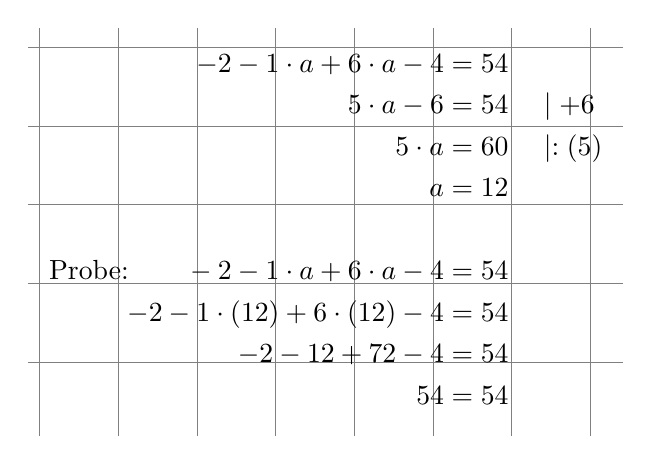
\begin{tikzpicture}[show background grid]
\node[below right] at (0,0.1) {
$\begin{aligned}
-2-1\cdot a+6\cdot a-4 &=54& &  \\
5\cdot a - 6 &=54& & \mid + 6\\
5\cdot a &=60& & \mid :\left(5\right)\\
a &=12& & 
\\
\\
\mbox{Probe:}\qquad -2-1\cdot a+6\cdot a-4 &=54& &  \\
-2-1\cdot \left(12\right)+6\cdot \left(12\right)-4 &=54& &  \\
-2-12+72-4 &=54& &  \\
54 &=54& &  \\
\end{aligned}$};
\end{tikzpicture}
\endgroup
&
r)&\begingroup\setlength{\jot}{-0.03cm}
\tikzstyle{background grid}=[draw, black!15,step=.5cm]
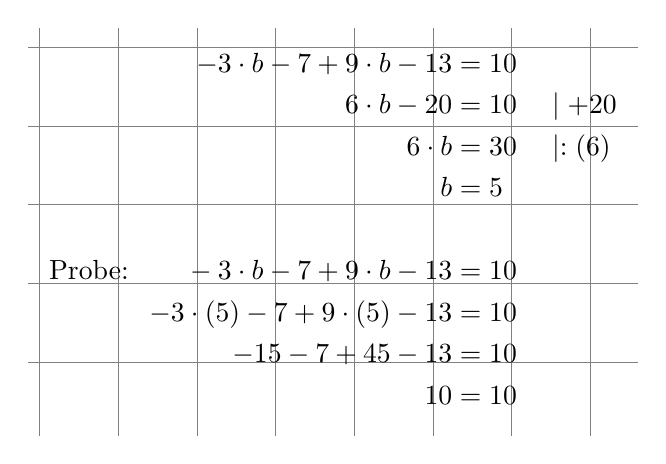
\begin{tikzpicture}[show background grid]
\node[below right] at (0,0.1) {
$\begin{aligned}
-3\cdot b-7+9\cdot b-13 &=10& &  \\
6\cdot b - 20 &=10& & \mid + 20\\
6\cdot b &=30& & \mid :\left(6\right)\\
b &=5& & 
\\
\\
\mbox{Probe:}\qquad -3\cdot b-7+9\cdot b-13 &=10& &  \\
-3\cdot \left(5\right)-7+9\cdot \left(5\right)-13 &=10& &  \\
-15-7+45-13 &=10& &  \\
10 &=10& &  \\
\end{aligned}$};
\end{tikzpicture}
\endgroup
\\\hline
s)&\begingroup\setlength{\jot}{-0.03cm}
\tikzstyle{background grid}=[draw, black!15,step=.5cm]
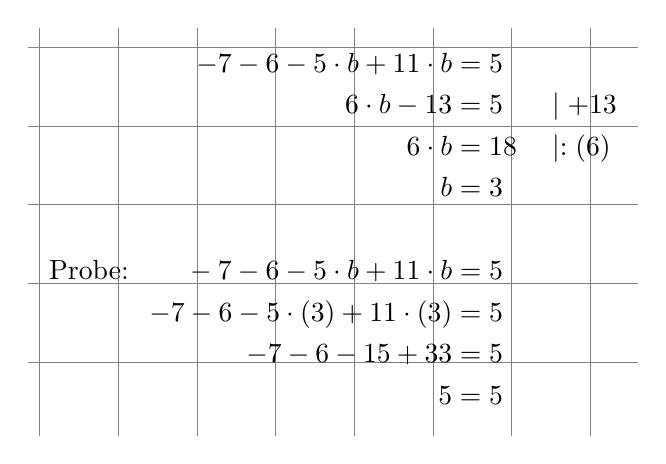
\begin{tikzpicture}[show background grid]
\node[below right] at (0,0.1) {
$\begin{aligned}
-7-6-5\cdot b+11\cdot b &=5& &  \\
6\cdot b - 13 &=5& & \mid + 13\\
6\cdot b &=18& & \mid :\left(6\right)\\
b &=3& & 
\\
\\
\mbox{Probe:}\qquad -7-6-5\cdot b+11\cdot b &=5& &  \\
-7-6-5\cdot \left(3\right)+11\cdot \left(3\right) &=5& &  \\
-7-6-15+33 &=5& &  \\
5 &=5& &  \\
\end{aligned}$};
\end{tikzpicture}
\endgroup
&
t)&\begingroup\setlength{\jot}{-0.03cm}
\tikzstyle{background grid}=[draw, black!15,step=.5cm]
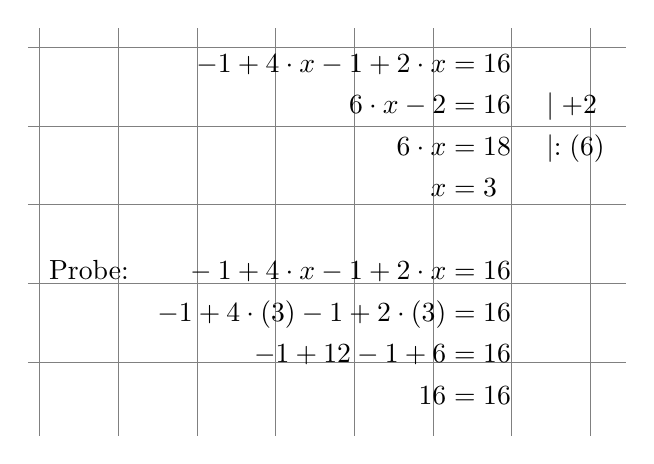
\begin{tikzpicture}[show background grid]
\node[below right] at (0,0.1) {
$\begin{aligned}
-1+4\cdot x-1+2\cdot x &=16& &  \\
6\cdot x - 2 &=16& & \mid + 2\\
6\cdot x &=18& & \mid :\left(6\right)\\
x &=3& & 
\\
\\
\mbox{Probe:}\qquad -1+4\cdot x-1+2\cdot x &=16& &  \\
-1+4\cdot \left(3\right)-1+2\cdot \left(3\right) &=16& &  \\
-1+12-1+6 &=16& &  \\
16 &=16& &  \\
\end{aligned}$};
\end{tikzpicture}
\endgroup
\\\hline
u)&\begingroup\setlength{\jot}{-0.03cm}
\tikzstyle{background grid}=[draw, black!15,step=.5cm]
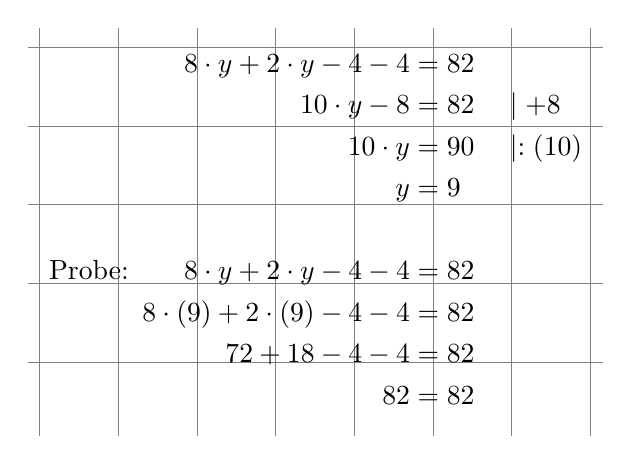
\begin{tikzpicture}[show background grid]
\node[below right] at (0,0.1) {
$\begin{aligned}
8\cdot y+2\cdot y-4-4 &=82& &  \\
10\cdot y - 8 &=82& & \mid + 8\\
10\cdot y &=90& & \mid :\left(10\right)\\
y &=9& & 
\\
\\
\mbox{Probe:}\qquad 8\cdot y+2\cdot y-4-4 &=82& &  \\
8\cdot \left(9\right)+2\cdot \left(9\right)-4-4 &=82& &  \\
72+18-4-4 &=82& &  \\
82 &=82& &  \\
\end{aligned}$};
\end{tikzpicture}
\endgroup
&
v)&\begingroup\setlength{\jot}{-0.03cm}
\tikzstyle{background grid}=[draw, black!15,step=.5cm]
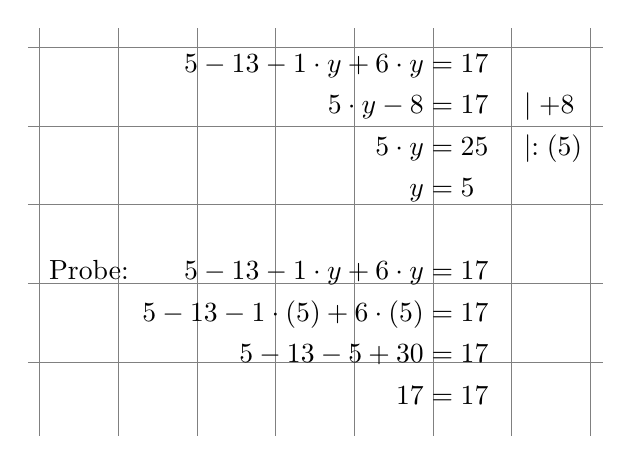
\begin{tikzpicture}[show background grid]
\node[below right] at (0,0.1) {
$\begin{aligned}
5-13-1\cdot y+6\cdot y &=17& &  \\
5\cdot y - 8 &=17& & \mid + 8\\
5\cdot y &=25& & \mid :\left(5\right)\\
y &=5& & 
\\
\\
\mbox{Probe:}\qquad 5-13-1\cdot y+6\cdot y &=17& &  \\
5-13-1\cdot \left(5\right)+6\cdot \left(5\right) &=17& &  \\
5-13-5+30 &=17& &  \\
17 &=17& &  \\
\end{aligned}$};
\end{tikzpicture}
\endgroup
\\\hline
w)&\begingroup\setlength{\jot}{-0.03cm}
\tikzstyle{background grid}=[draw, black!15,step=.5cm]
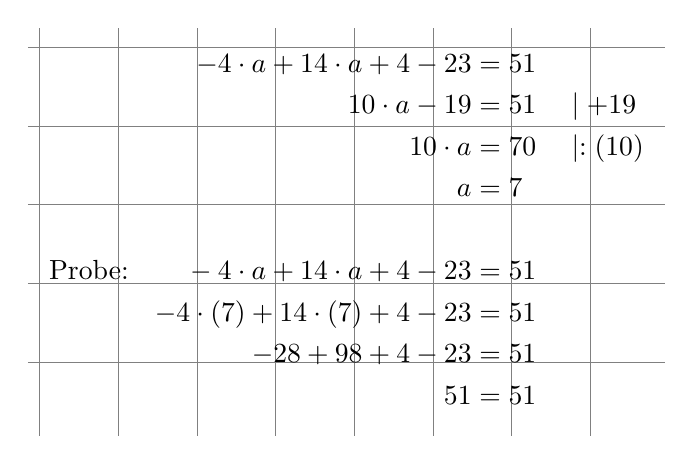
\begin{tikzpicture}[show background grid]
\node[below right] at (0,0.1) {
$\begin{aligned}
-4\cdot a+14\cdot a+4-23 &=51& &  \\
10\cdot a - 19 &=51& & \mid + 19\\
10\cdot a &=70& & \mid :\left(10\right)\\
a &=7& & 
\\
\\
\mbox{Probe:}\qquad -4\cdot a+14\cdot a+4-23 &=51& &  \\
-4\cdot \left(7\right)+14\cdot \left(7\right)+4-23 &=51& &  \\
-28+98+4-23 &=51& &  \\
51 &=51& &  \\
\end{aligned}$};
\end{tikzpicture}
\endgroup
&
x)&\begingroup\setlength{\jot}{-0.03cm}
\tikzstyle{background grid}=[draw, black!15,step=.5cm]
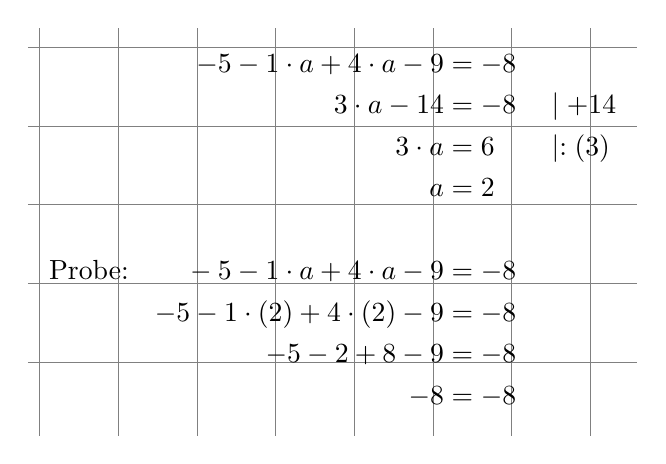
\begin{tikzpicture}[show background grid]
\node[below right] at (0,0.1) {
$\begin{aligned}
-5-1\cdot a+4\cdot a-9 &=-8& &  \\
3\cdot a - 14 &=-8& & \mid + 14\\
3\cdot a &=6& & \mid :\left(3\right)\\
a &=2& & 
\\
\\
\mbox{Probe:}\qquad -5-1\cdot a+4\cdot a-9 &=-8& &  \\
-5-1\cdot \left(2\right)+4\cdot \left(2\right)-9 &=-8& &  \\
-5-2+8-9 &=-8& &  \\
-8 &=-8& &  \\
\end{aligned}$};
\end{tikzpicture}
\endgroup
\\\hline
y)&\begingroup\setlength{\jot}{-0.03cm}
\tikzstyle{background grid}=[draw, black!15,step=.5cm]
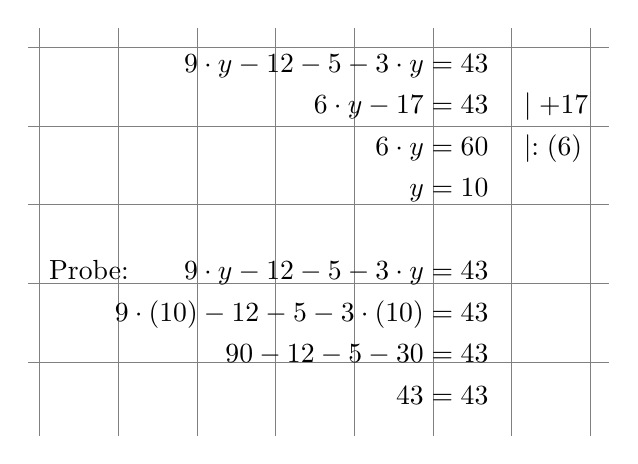
\begin{tikzpicture}[show background grid]
\node[below right] at (0,0.1) {
$\begin{aligned}
9\cdot y-12-5-3\cdot y &=43& &  \\
6\cdot y - 17 &=43& & \mid + 17\\
6\cdot y &=60& & \mid :\left(6\right)\\
y &=10& & 
\\
\\
\mbox{Probe:}\qquad 9\cdot y-12-5-3\cdot y &=43& &  \\
9\cdot \left(10\right)-12-5-3\cdot \left(10\right) &=43& &  \\
90-12-5-30 &=43& &  \\
43 &=43& &  \\
\end{aligned}$};
\end{tikzpicture}
\endgroup
&
z)&\begingroup\setlength{\jot}{-0.03cm}
\tikzstyle{background grid}=[draw, black!15,step=.5cm]
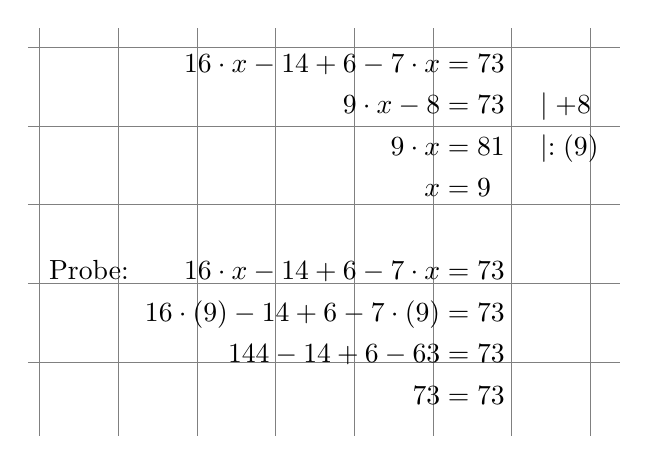
\begin{tikzpicture}[show background grid]
\node[below right] at (0,0.1) {
$\begin{aligned}
16\cdot x-14+6-7\cdot x &=73& &  \\
9\cdot x - 8 &=73& & \mid + 8\\
9\cdot x &=81& & \mid :\left(9\right)\\
x &=9& & 
\\
\\
\mbox{Probe:}\qquad 16\cdot x-14+6-7\cdot x &=73& &  \\
16\cdot \left(9\right)-14+6-7\cdot \left(9\right) &=73& &  \\
144-14+6-63 &=73& &  \\
73 &=73& &  \\
\end{aligned}$};
\end{tikzpicture}
\endgroup
\\\hline
\end{xltabular}
\vspace{0.5cm}
\end{document}